\section{Brief Overview}
In a world where the demand for high performance hand-held computing devices continues to grow and the prevalence of ``smart'' devices is increasing, there is unprecedented demand for \ac{SOC} devices to control systems as varied as medical devices and entertainment systems.
As these applications become more and more demanding, with ever increasing amounts of data to process and the expectation that today's devices will outperform those of yesterday, the problem of maintaining the steady gain in performance of \acp{SOC} remains at the fore.

The main drivers of performance in \acp{SOC} are the number of transistors on a chip, which is correlated with the number of calculations that can be carried out simultaneously, and the frequency at which the device operates, which determines the number of calculations performed per second.
Moore's Law, based on the famous observation by Gordon Moore in 1965\cite{moore1965cramming}, predicted a doubling in the transistor count of \ac{IC}s per year for the forthcoming decade. This behaviour has carried on to this day as a result of the ever decreasing size of transistors, and has only begun to slow down in recent years.
However, as the number of transistors on a chip has increased roughly following Moore's Law, the increase in clock frequency has not been able to follow a similar linear trajectory, having remained roughly equivalent for the last number of years \cite{ross2008cpu}, indeed the clock speed of the Intel Core family of \ac{CPU}s has not changed since their introduction in 2009 \cite{intelark}.
\begin{figure}[h]
	\centering
	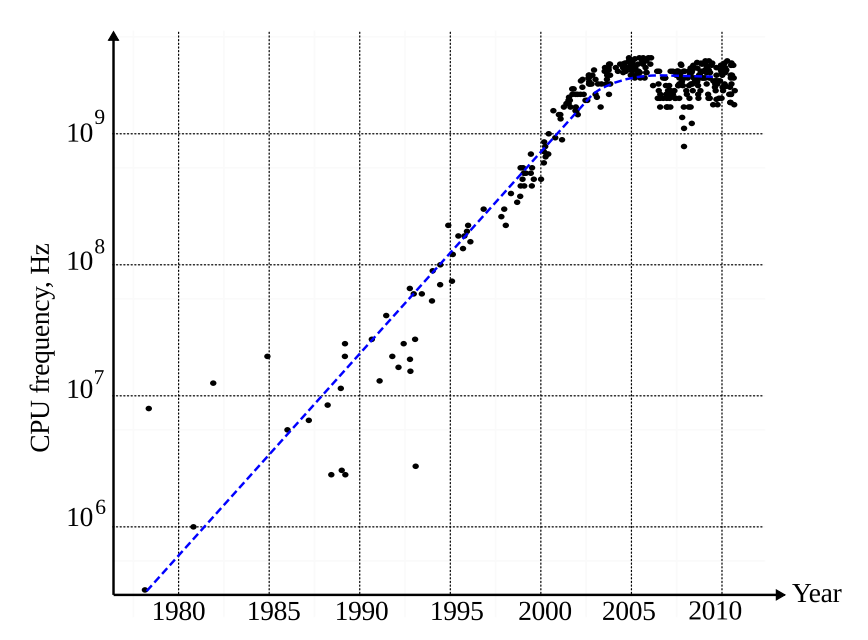
\includegraphics[scale=0.4]{../eldar_last_30_yrs}
	\caption{Frequency of the Intel microprocessors over past 30 years \cite{zianbetov2013phd}.}
	\label{fig:eldar_last_30_yrs}
\end{figure}\\
This plateauing of clock frequency has been caused by high power consumption due to the demands placed by the global distribution of a high frequency clock, often the single biggest consumer of power on the chip \cite{tiwari1998reducing}.
With the growth of the \ac{IOT} market where low power devices are desirable, with many of the emerging uses of \ac{SOC}s being portable and thus without a permanent power source, high power consumption goes directly against one of the key pillars of the technology. This forces many of these devices to use lower performance hardware in order to reduce the power consumption, and increase the battery life, of their devices.

In digital systems, two main approaches are used when designing the clocking system. In both cases, the chip is broken down into small areas in which all transistors are clocked synchronously, with the size constrained by the ability to deliver a quality clock signal to all transistors. The first of these methods is \ac{GSLS}, where the clock signals in each of these subregions of the chip are synchronised with one other. In practice, however, this is very difficult to achieve, as extremely high precision is required across the ever increasing number of transistors and the entire area of the chip, and doing so leads to high power consumption.

In contrast in a \ac{GALS} clock delivery system the ``local'' areas are not synchronised with other. This reduces the clocking system's complexity and thus the power consumption and chip area used, at the expense of communication speed between blocks. This disadvantage comes from the need to then somehow synchronise the messages being sent from one area to another to avoid the corruption of any messages.
A \ac{GSLS}, system, however has the advantages of deterministic behaviour and greater rates of communication between clocking areas and, as such, remains a desirable system design. A number of methods which deliver \ac{GSLS} clocking exist at present such as clock trees as well as emerging technologies such as ADPLL networks.

\section{The Impact of Clocking Errors}
In Figure \ref{fig:eldar_why_precise_clocking} the data path between two synchronously clocked registers is shown, with the circuit's function being carried out by the combinatorial network between the registers.
Each register has a setup time, which represents the amount of time that the input value to a register must remain constant before the clock edge, and a hold time, the time for which the input must remain constant after a clock edge.
\begin{figure}[h]
	\centering
	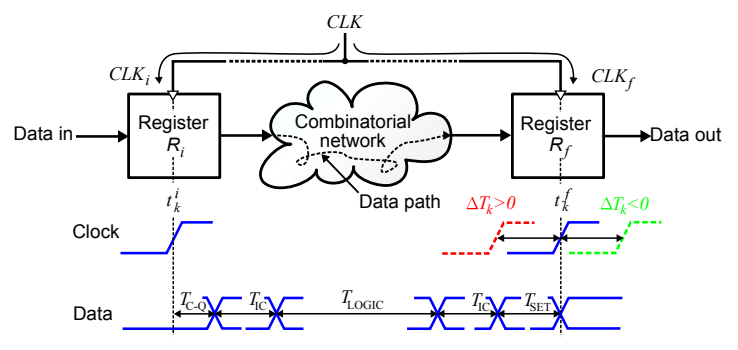
\includegraphics[scale=0.6]{../eldar_why_precise_clocking}
	\caption{Data Flow in a Clocked System \cite{zianbetov2013phd}.}
	\label{fig:eldar_why_precise_clocking}
\end{figure}

A lack of synchronisation between the clock edges will manifest itself as a time difference between the clocking events at both registers, $\Delta T = t^i_k - t^f_k$. $\Delta T$ is considered to be ergodic and can be described by an average deviation called skew and random process, normally modelled as a Gaussian random variable. If $\Delta T$ is negative this reduces the time available for the intervening combinatorial network thereby, having the same effect as a reduction in clocking frequency. Correspondingly a positive $\Delta T$ for depicted registers implies a negative $\Delta T$ for $R_f$ and the subsequent register. 
The most common sources of clock error are caused by mismatches which usually stem from production, such as differences in the length of clocking paths, buffer delays or in the parameters of either active or passive components in the clock distribution network, which as the size of components on an \ac{IC} reduces becomes more difficult to avoid. All sources of mismatch will manifest themselves in the clock distribution system as skew between transistors, while the noise in active components or the power supply system will appear as jitter in the clock signal.

\section{Traditional Solutions}
A number of traditional solutions exist which provide \ac{GSLS} clocking systems, using a variety of techniques. The most simple of these implement clock distribution systems that are symmetrical in order to distribute a centrally generated clock signal to all areas of the chip at the same phase. These systems are named in accordance with their geometry, with the most common variants being branch, X or H trees. 
\begin{figure}[h]
	\centering
	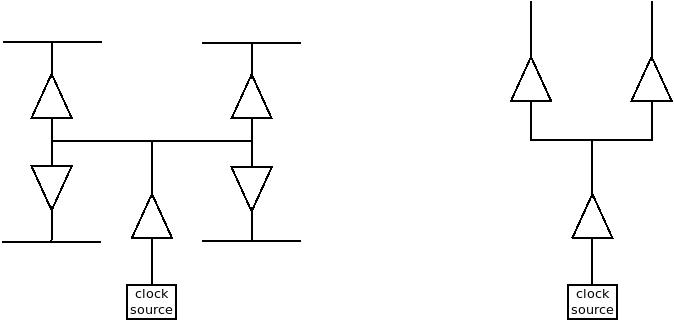
\includegraphics[scale=0.33]{../trees}
	\caption{H and Branch Tree Clock Distribution Systems.}
	\label{fig:trees}
\end{figure}

While on the surface these appear simple, the task of obtaining an exact matching is, in practice, the limiting factor in this design. Even if the clock distribution system is geometrically symmetrical by design, production mismatches in either active or passive components will lead to a skew that varies from part to part. In order to minimise the impact of production tolerances, the dimensions of components in the distribution network can be increased, thus reducing the relative variation possible. However this has the impact of increasing the power consumption of the distribution network \cite{tiwari1998reducing}.

A mesh clock distribution network is an alternate design where the clock is delivered using a Cartesian grid of distribution lines. Compared to a tree type system, the variation in skew seen with a clock mesh is inversely proportional to the density of the grid while the sources of jitter remain identical. According to Abdelhadi \textit{et al} (2010) clock meshes ``\textit{achieve low and deterministic skew, low skew variations, and low jitter}'', all desirable characteristics for a clock distribution system. However they dissipate more power due to extra capacitive loading, attributable to vast number of lines required to form the grid. Similarly mesh distribution networks suffer from potential mismatch in production and alleviation through increasing of the dimensions of interconnects will, as with a tree type system, lead to higher power consumption \cite{abdelhadi2010timing}. 
\begin{figure}[h]
	\centering
	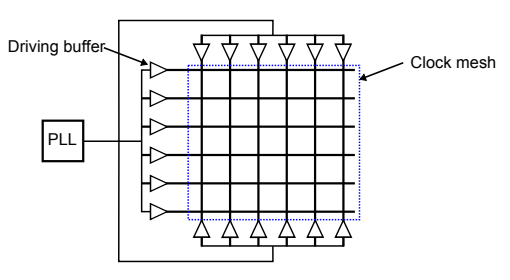
\includegraphics[scale=0.7]{../tex_files/eldar_mesh}
	\caption{Mesh Clock Distribution System \cite{zianbetov2013phd}.}
	\label{fig:mesh}
\end{figure}
Alternative designs replace the electrical lines used in the tree networks with waveguides for optical signals, with only the distribution in the local area carried out using regular wires. This technique presents many advantages \cite{chen2006chip}: optical clock delivery is immune to the noise sources that affect electrical clock distribution systems, consume less power and do not suffer from the electrical losses present in a regular tree system.

\section{Skew Compensation}
In a tree type distribution system, skew is the main issue affecting clock accuracy and as such some effort has gone into addressing the problem. Skew due to the manufacturing process can be, at least, partly accounted for by means of active control through a skew compensator. This is a circuit, or controller, that compares the skew of each local clocking area on the chip and attempts to ensure in-phase clock delivery. Two main strategies exist to provide skew compensation, each named according to the location of the control mechanism. Designs featuring the controller located at the clock source, are known as ``centralised'' methods, and those with multiple controllers in the individual clocking areas known as ``decentralised''. Regardless of the controller placement these techniques allow for the tuning of the propagation delay between the centralised clock source and the local clocking areas.

In a centralised skew compensation circuit, the skew across the chip is calculated by the central controller which then manipulates the distribution network in order to deliver a more in-phase clock around the chip. This calculation is done by measuring the round trip time from the clock source to both the root of local clock tree, and to the individual ``leaves'' of the tree. The controller then has a limited ability to tune the propagation path. The downsides of this technique are the resolution of both the measurement and compensation are poor, allowing for the correction of just skew and not of any jitter that may be present in the system, and that the extra circuitry required for both the tunability of the forward path and the two extra return paths contribute to an increased footprint and power consumption.

As the name suggest a decentralised skew compensation technique delegates the responsibility of tuning the propagation path to the individual clock regions. This strategy has the advantage of not requiring the return paths present in a ``centralised'' design. Instead comparison is made betweeen the leaves of different clocking areas and on this basis the propagation delay is varied.
For example, Yamashita \textit{et al} (2005) designed a system in which each clocking area or ``leaf node'' contains a partial clock tree. Each of these ``leaves'' is able to compare its clock phase to the neighbouring node, and based on the result, tune an adjustable delay buffer \cite{yamashita2005dynamic}. While this method can compensate for process, voltage and temperature variation, it does not address the power consumption due to the delivery of a high frequency clock across the entire chip area nor does it have any impact on clock jitter.

%DOWN TO HERE DONE FOR ACRO
\section{Multi-oscillator Designs}
The designs described previously, are all similar in that they have a single central oscillator that provides the clock for all areas of the chip, whereas the following methods attempt to synchronise multiple oscillators, each of which provides the clock for a single clocking area. The main advantages of a multi-oscillator design, are that as each clocking area has its clock created locally, there is no degradation in the quality of the signal as it is distributed around the chip and the number of potential noise sources is reduced. In order to obtain global synchronisation some method of comparison between local clocking areas is required, and how this is done depends on the architecture. Regardless of the comparison is made, it is carried out between neighbouring clocking areas and as such the feedback network need not have a large footprint or power overhead.

One such method is a network of oscillators as in Figure \ref{fig:mizuno1998noise} which uses coupled \ac{PLL} to generate local clocks. Here the output of a leaf node is compared with an external reference and the operating frequency of each \ac{VCO} tuned based on the result.
\begin{figure}[h]
	\centering
	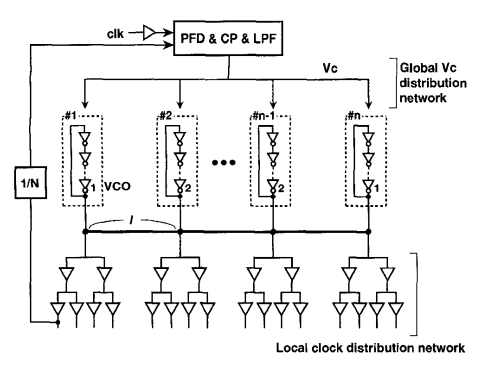
\includegraphics[scale=0.7]{../mizuno1998noise}
	\caption{Coupled Oscillator Clock Delivery Circuit \cite{mizuno1998noise}.}
	\label{fig:mizuno1998noise}
\end{figure}
The advantage of this method is the simplicity of the feedback network, requiring just the divided clock output from a single leaf node. The \ac{VCO}s then adjusted by the control voltage, $v_c$, which needs delivery to all areas of the chip. However, this is a regular signal and as such does not suffer from skew or jitter. This alleviates the need for a power hungry distribution circuit, while also being more noise-immune than the transmission of a high frequency clock. However this design still suffers from clock variation as all \ac{VCO}s are fed the same control voltage, and thus the manufacturing tolerance issues present in conventional designs persists here also. This is acknowledged by the authors:
\begin{quotation}
	\textit{Unfortunately, as with the conventional ... method, distributing the \ac{VCO}s over the entire chip causes the problem that jitter and skew are increased by variations in the fabrication process (static), temperature, and power supply (dynamic)} \cite{mizuno1998noise}.
\end{quotation}
This type of multi-oscillator design is implemented by analogue circuits, and as a result not only are the clock signals, but also the control signals are liable to variation due to noise, fabrication mismatch and power supply dynamics.

Another potential multi-oscillator clock distribution system uses the phase relationship between the oscillators driving neighbouring clock areas in order to obtain synchronisation. Once again, this negates the requirement for a global distribution structure and the signals used for comparisons need only be sent between neighbouring clocking areas. As a \ac{PLL} is being used it is again possible to perform the phase comparisons using a divided version of the generated clock. This in turn means the hardware transporting the divided clock signal to the phase comparator, has significantly lower requirements placed on it, thus lowering the power consumption due to electrical losses. Pratt and Nguyen initially proposed method of clock distribution in their 1995 paper entitled ``\textit{Distributed Synchronous Clocking}'' in which they propose a Cartesian grid of clocking areas, each with their own \ac{PLL}, which has become known as a \ac{PLL} Network \cite{pratt1995distributed}. In this design any given node is synchronised with its neighbours and one of the corner nodes is additionally synchronised with the reference. According to the authors this is ``a simple, effective way to achieve low cost, high quality, low skew clock generation in a synchronous parallel processor''. They did, however, note the presence of a phenomenon called ``mode locking'', which is setting of the network into a stable equilibrium where there are non-zero relative phases.

\begin{figure}[h]
	\centering
	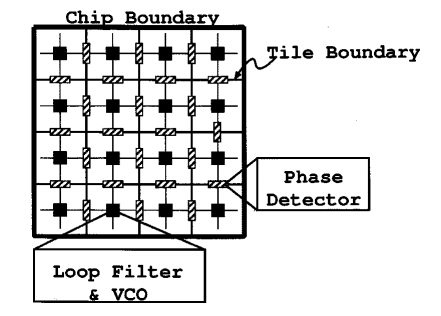
\includegraphics[scale=0.7]{../gutnik2000active}
	\caption{PLL Network Topology \cite{gutnik2000active}.}
	\label{fig:gutnik2000active}
\end{figure}

This architecture of clock distribution network was then implemented by Gutnik \textit{et al} (2000) who fabricated a 4x4 array of oscillators, operating at a centre frequency of 1.2 MHz. The oscillator was implemented as a voltage controlled ``nMOS-loaded differential ring oscillator'', and in order to mode locking the phase detector was implemented as a highly non-linear circuit. The design was a success and the authors concluded:
\begin{quote}
	\textit{Design and measurements on this chip confirm that generating and synchronizing multiple clocks on chip is feasible. Neither the power nor the area overhead of multiple \acs{PLL}s is substantial compared to the cost of distributing the clock by conventional means} \cite{gutnik2000active}.
\end{quote}

The remaining benefits of such a clock distribution system are: As the individual oscillators have their own control signal mismatch between different oscillators is not a factor as they will also receive different control signals. Secondly, and unlike the conventional methods, sources of jitter in the system such as power supply dynamics can be accounted for. Finally symmetry between the different oscillators is not required, once again attributable to the individual control signals in use. 
\section{ADPLL Networks}
As a \ac{PLL} network is an analog circuit, its integration in a modern \ac{IC} is a barrier to usage, and as such it has not been used in any commercial designs \cite{zianbetov2013distributed}. An alternative design that is more suitable for current fabrication techniques eschews from using analogue components and instead implements the network of controlled oscillators using only digital circuitry, hence the name All-Digital \ac{PLL}. A 4x4 \ac{ADPLL} network was designed and prototyped in 65 nm CMOS by Zianbetov and Shan in order to test the suitability of the technique as a clock distributor \cite{zianbetov2013phd,shan2014phd}.

In this design the oscillators are once again laid out in a Cartesian grid, with each node coupled to their neighbours in phase. As this is now a digital system the coupling is carried out using digital phase comparators, which attempt to measure the phase difference between two oscillators. Figure \ref{fig:eldar_node} shows high level detail of the architecture of both the entire clocking system and that of an individual node in the design. The digital nature of this architecture brings with it a number of advantages over traditional analogue implementations, as it can benefit from advancements in digital circuit design suites, be reconfigurable and programmable and has a significantly greater immunity to perturbations inherent to its digital nature, as the exact voltage of signals is of no importance \cite{zianbetov2013phd}. This last advantage is of particular use in a digital environment, as otherwise there is potential for clock degradation resulting from switching of transistors. The drawback of the switch to a digital architecture however is the presence of quantisation. Analogue designs both deliver continuous control signals to the oscillators and have a continuous phase detection capability, unlike a digital system where these actions are carried out with fixed resolution.
\begin{figure}[h]
	\centering
	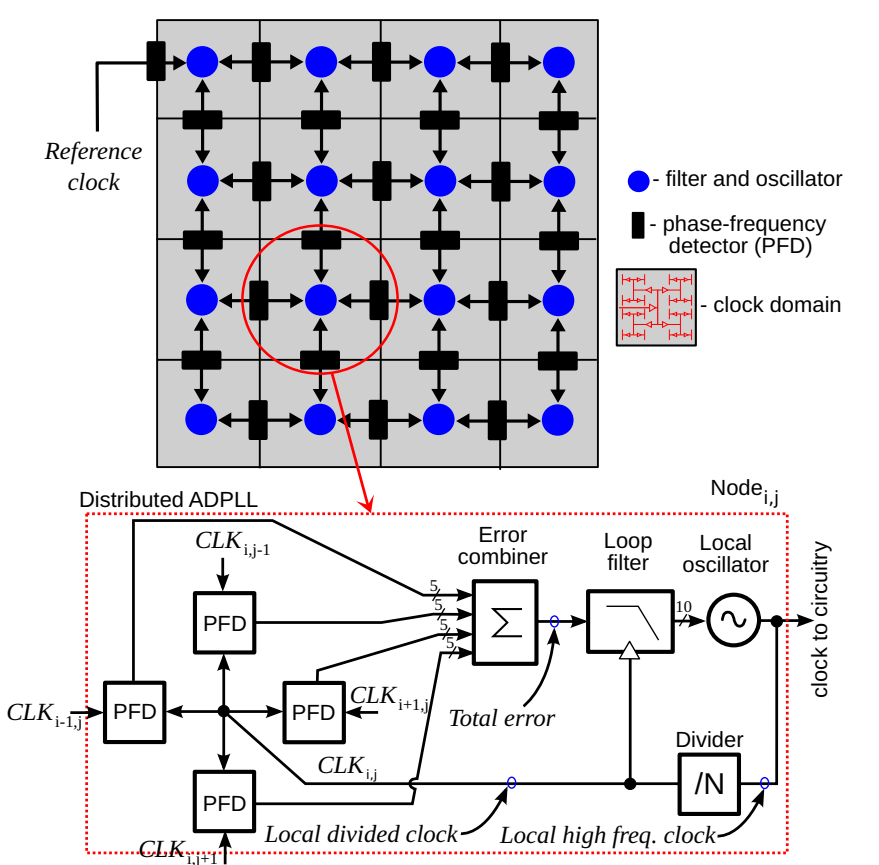
\includegraphics[scale=0.4]{../ccirc_2013_arch}
	\caption{Architecture of the ADPLL network and of a single node \cite{zianbetov2013distributed}.}
	\label{fig:eldar_node}
\end{figure}

Looking at the design of a given node it is notable that the function carried out by the Error Combiner is akin to a average, therefore as mentioned by Pratt and Nyugen, there is potential to a mode locked equilibrium in which the oscillators are not synchronised. In their paper, they presented a method where initial start-up was performed uni-directionally and, once all nodes are close to alignment, full connectivity could be restored, however this was not viable in an analogue system as reconfigurability was not an option \cite{pratt1995distributed}. In creating an entirely digital system, Zianbetov and Shan could exploit reconfigurability and implement a uni-directional start-up and thus avoid the problem of convergence into a mode locked state, without having to design a non-linear phase detector.

\section{\acl{ADPLL} Architecture}
As indicated in Figure \ref{fig:mulkeen_pll} the three main building blocks of a conventional \ac{PLL} are the \ac{PD}, \ac{LF} and \ac{VCO}. In an \ac{ADPLL} these blocks are then replaced by their digital counterparts, necessitating quantisation in order to remain physically realisable. The ``All-Digital'' moniker is a misnomer as the oscillator and \acl{PD} are usually both implemented by mixed signal circuits.
\begin{figure}[h]
	\centering
	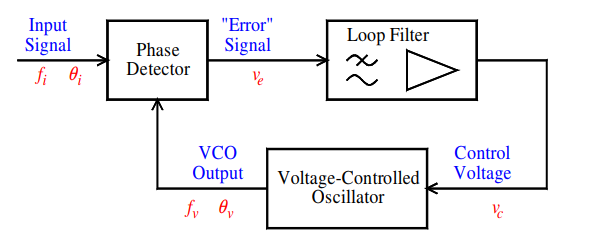
\includegraphics[scale=0.5]{../tex_files/mulkeen_pll}
	\caption{Block Diagram of a \acl{PLL}, \textit{Wireless Systems Notes}, B. Mulkeen (2017).}
	\label{fig:mulkeen_pll}
\end{figure}

\subsection{Digitally Controlled Oscillator}
In a digital system there are a very limited number of voltages representable, most commonly just two, so using a voltage to control the oscillator is not a viable strategy. Instead a fixed bit width signal is used to control the oscillator's period, selecting the number of inverters in a ring oscillator or the varactor configuration of a travelling wave oscillator \cite{chen2011rotary}. The decisions made in the design of the \ac{DCO}, or \ac{NCO}, determine many of the other \ac{ADPLL} parameters. While tuning range and centre frequency, as well as linearity, carry over from the analogue counterpart, a \ac{DCO} also has a frequency step which in combination with the bit width of the control signal determines the range over which the oscillator can be tuned. Figure \ref{fig:my_ring} illustrates a basic ring oscillator design. A ring oscillator is an inherently unstable circuit composed of an odd number of inverters connected in a circle, which allows a signal to propagate infinitely, with the signal at any point in the circuit appearing as a square wave. The half-period of this oscillator is the time taken for the signal to propagate once through the chain, $n$ times the propagation delay through one inverter. The frequency of operation can then be set by modulating the length of the chain, in steps of two inverters to maintain an odd number, by means of \texttt{f\_select}. The main impact of output frequency quantisation is that only frequencies which are integer multiples of the frequency step away from the centre frequency can be easily reproduced, with intermediate values only obtainable in a manner akin to Fractional-N synthesis with the control code toggling back and forth. This acts as a source of jitter in the system.
\begin{figure}[h]
	\centering
	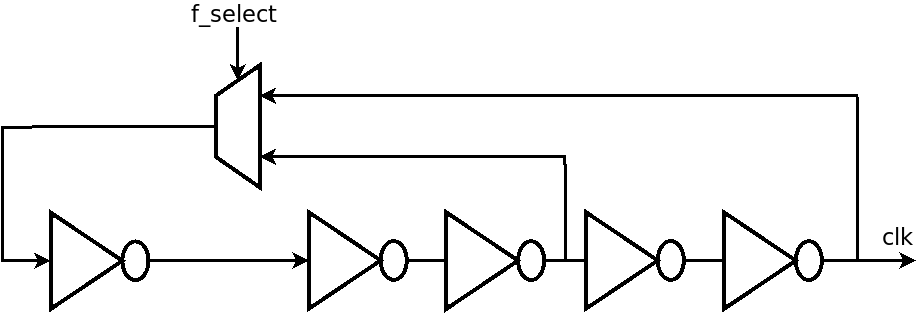
\includegraphics[scale=0.275]{../inverter_chain}
	\caption{Basic Ring/Inverter Chain Oscillator.}
	\label{fig:my_ring}
\end{figure}

It is also possible to implement an \ac{NCO} by means of a counter, in a manner that will produce either linear period or linear frequency steps. Both methods use the most significant bit of the counter's value to form the output signal. Period linearity is achieved by varying the reload value of the counter after overflow depending on the control code, thereby changing the period by a multiple of a fixed step. Alternatively frequency linearity can be achieved if the reload value is left constant, but instead the amount added to the counter every clock cycle is changed according to the control code, once again a fixed step size is used.

\subsection{Digital Phase Detector}
Once again quantisation impacts the \acl{PD}, as rather than a continuous output the phase detector in an \ac{ADPLL} has a finite number of output values, thus limiting the accuracy of the phase detector. A second form of quantisation is also present, as unlike an analog system, a digital phase detector does not provide continuous data in the time domain either, instead relying on sampling. At its most basic, a digital phase comparator may only output an indication of which signal is leading, a design known as a Bang-Bang Detector, which can be constructed using a single D Flip Flop with one the generated signal connected to the ``D'' input and the reference signal acting as the clock. As the output only has two levels the resultant word is only 1 bit wide and as such, limits the range over which the output frequency can be controlled. More complex designs such as that in Figure \ref{fig:shan_bb_pd}, implemented by Shan, build on this by measuring the time difference between edges of the signals using a \ac{TDC} in his case using a \ac{TDL} \cite{shan2014phd}. A \ac{TDL} is constructed by a chain of elements of a fixed delay, and the signal to be timed is applied to this start of this chain. After the timing interval elapsed the values at each point in the chain are examined, and using temperature coding, these are converted to a digital signal, the width of which is the bit width of the \ac{PD}'s error signal. This mimics a time measurement and allows for the phase difference to be recorded in a non binary manner.

\begin{figure}[h]
	\centering
	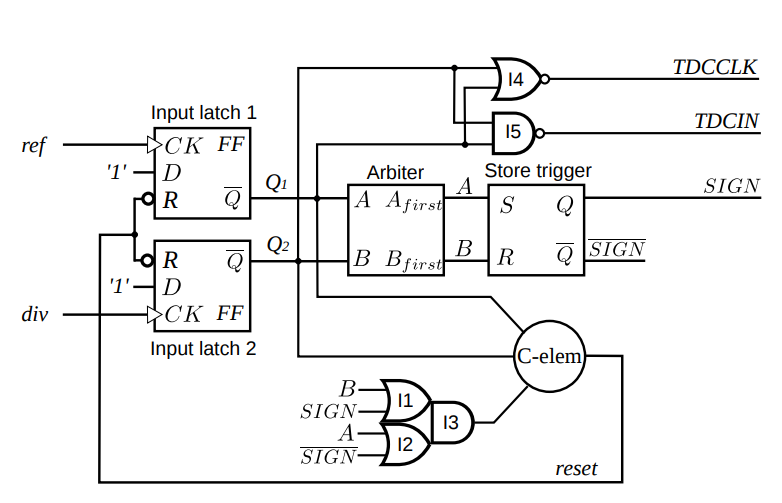
\includegraphics[scale=0.35]{../shan_bb_pd}
	\caption{Bang-bang phase/frequency detector architecture. \cite{shan2014phd}.}
	\label{fig:shan_bb_pd}
\end{figure}

\subsection{Digital Loop Filter}
\begin{figure}[h]
	\centering
	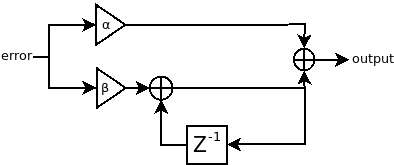
\includegraphics[scale=0.45]{../pi_simple}
	\caption{Basic PI Controller Architecture.}
	\label{fig:my_simple_pi}
\end{figure}%TODO ask mulkeen if this is IIR
The \acl{LF} in an \ac{ADPLL} can be implemented as a \ac{PI} controller, as only a low-pass filter is required, such as that in Figure \ref{fig:my_simple_pi}. In the case of a node in an \ac{ADPLL} network the input of this filter is a weighted of the phase difference relative to the neighbouring local clocking areas. In one example topology a digital system the proportional section can be implemented by a simple multiplier, whereas the integral path is constructed by adding the result of a multiplication by the proportional gain to an accumulator. This delayed summation can be easily implemented by an accumulator to which the current value of the multiplication is added each cycle, and as such the system has an infinite impulse response. The value of these gains determine the response and stability of the \ac{ADPLL} network. The transfer function of such a controller is given by \cite{shan2014phd}:
\begin{equation*}
	H(z) = \alpha + \beta\frac{1}{1-z^{-1}} = \frac{(\alpha + \beta) - \alpha z^{-1}}{1-z^{-1}}
\end{equation*}
It has been found by Koskin \textit{et al} (2018) that stable operation can be achieved when the integral gain, $k_i$, is less than half the proportional gain, $k_p$ \cite{koskin2018generation}. In the same study a range of values was found which would produce low jitter operation of the network. As these values are all less than one, the filter must implement fixed point arithmetic in an effort to maintain the simplicity of the clock distribution network, rather than incurring the complexity penalty of floating point calculations.

\subsection{Error Combiner}
The \ac{ADPLL}s used in a network need to combine the error signals from multiple neighbours to determine what the average difference from its neighbours is, and this necessitates the addition of the Error Combiner. In a digital system this can be implemented by a weighted average of the different error signals, with the weight being modifiable at run-time. This configurability is what permits the system to implement uni-directional mode and also allows for the weighting applied to certain signals, such as the external reference, to be modified. The ease of implementation of a configurable error combiner is one of the main advantages of an \ac{ADPLL} over an analogue system.

\section{The Role of the FPGA}
A \acl{FPGA} is a type of \ac{IC} that is designed to be configured by a designer after the chip itself has been manufactured. An \ac{FPGA} contains a large number of logic elements that can be connected together in order to perform complex logic, written using the same \ac{HDL}s used to design the digital blocks of \ac{ASIC}s. They may also implement started modules such as adders, multiplexers and \ac{RAM} as a fundamental element. More complex logic is often implemented using multiplexed lookup tables rather than true logic elements. High end devices such as the Xilinx Zynq Ultrascale even implement Multi-Processor \ac{SOC}s. Compared to an \ac{ASIC} the designer does not have direct control over the layout of the system but rather describes its behaviour, possibly down to the basic logic elements of inverters or other gates. Limited control is possible over the placement of the individual modules, but \ac{EDA} tools are responsible for the exact placement of elements. As a result, it is not possible to have precise control over the delays experienced as signals propagate through the design. To assist with the resolution of any issues \ac{EDA}s provide tools to analyse timing behaviour.

Prototyping on an \ac{FPGA} is a common verification stage for conventional \ac{ASIC} designs as it allows for a hardware validation of any digital circuitry, and the detection of any potential flaws or errors made by the design before the expensive of an \ac{ASIC} implementation. In their 2013 \ac{ADPLL} network implementation Zianbetov and Shan used an \ac{FPGA} in order to validate their programming interface, the design of the error processing block, ensure they had eliminated mode locking behaviour and to ensure phase synchronisation was possible \cite{zianbetov2013phd,shan2014phd}. However they experienced two main limitations, they were not able to implement the mixed-signal \ac{PFD} and \ac{DCO}, and the maximum frequency of operation possible was orders of magnitude lower than the GHz range of their \ac{ASIC} implementation. These issues were circumvented by implementing an alternative \ac{PFD} and \ac{DCO} designs which were driven by the clock distribution network provided by the \ac{FPGA} and every clock frequency scaled by the same amount such that the results of testing would remain indicative. One of the main advantages they saw was that the hardware description used for the digital blocks of their \ac{ASIC} could be directly ported over to the \ac{FPGA}.

It is however possible to implement limited mixed-signal circuits on an \ac{FPGA} through the use of primitive logic elements, however, as control over the implementation is restricted to the module level it is not possible to mirror the implementation of a design intended for an \ac{ASIC}. As these implementations are analogous to a mixed-signal circuit on an \ac{ASIC}, the verification of theoretical behaviours, as done by Koskin \textit{et all}, in order to test the findings of his PhD thesis \cite{theboys2019}, is made possible without the expense of \ac{ASIC} fabrication. An \ac{FPGA} based mixed-signal \ac{ADPLL} network is also seeing use here in \ac{UCD} as a initial prototyping platform for the validation of new modules for use in \ac{ASIC} based \ac{ADPLL} networks.

\ac{FPGA}s have been used in other fields to simulate and experiment with new technologies, although not all of these attempt to implement the mixed-signal circuitry using primitive elements. Fernandez-Alvarez \textit{et al} (2016) proposed a method suited to higher end \ac{FPGA}s in which a co-processor on the \ac{FPGA} simulates the mixed-signal circuitry while the digital section of the design is implemented on the \ac{FPGA} itself \cite{fernandez2017hw}. While the interfacing between hardware and software remains a challenge they found:
\begin{quotation}
	Obtained data are compared to the data obtained by means of using PSIM and ModelSim co-simulation. The proposed solution speeds up the evaluation in around one order of magnitude keeping the accuracy. The output signal differs in less than 0.6 mV (RMSD).
\end{quotation}

Mixed-signal circuits were, however, simulated in hardware by \'{O}scar Luc\'{i}a \textit{et al} (2011) on an \ac{FPGA} in order to overcome the excessive time penalty imposed by software based simulations that required the behaviour of both a digital and mixed-signal peripheral and that of a micro controller running code in C to be simulated side by side \cite{lucia2011real}. They concluded
\begin{quotation}
	... the proposed system provides a versatile and fast method to develop ad hoc control architectures, avoiding the need for time-consuming mixed-signal simulations and the risk of damaging the actual power converter implementation.

\end{quotation}
By carrying out simulations on an \ac{FPGA}, Guanhua Wang \textit{et al} (2013) achieved a 3000 times decrease in run-time when compared to an identical simulation in MATLAB used for the verification of a calibration algorithm for successive approximation analogue-to-digital converters \cite{wang2013fast}. Many other examples exist of \ac{FPGA}s used for the simulation of mixed-signal or \acl{RF} circuits in literature.
%TODO Elena had suggestions?

\section{\acs{ADPLL} Performance Characterisation}
As already stated, goal of a clock distribution system is to synchronise clocking events in all areas of the chip. The effectiveness of this synchronisation is characterised by two main metrics, jitter and skew, which together describe the distribution of clocking events. Skew is the average time delay between a clocking event in one area of the chip and that of a reference event. It can be easily measured by computing the average value of this delay. Jitter has a number of definitions depending on how it is measured, but at its most basic it is the standard deviation of the time delays with respect to the reference clocking edge.

The simplest form of clock performance characterisation is on a \ac{C2C} basis, in which the reference is the signal under test itself. Here the standard deviation of the individual periods gives the jitter of the signal, while skew has no meaning with a self reference the mean period can be used to compute the centre frequency over the time interval. For a more informative measurement the \ac{TIE} can be computed, which takes into account another signal as the reference. \ac{TIE} is calculated by comparing the delay between the signal in question and a reference that is treated as ideal. The mean value gives the relative skew between the two signals and once more the standard deviation of the measurements gives the jitter with respect to this reference.

Both above forms of measurement assume a large number of sequential measurements, however, there are other ways that jitter and skew can be calculated \cite{AN007}. Phase jitter is an important characteristic for communications systems as it can be used to calculate phase noise, important to ensure spurious emissions are within regulations. Long term, or accumulated, jitter represents the cumulative effect of jitter on the signal over several cycles. Long term jitter in particular affects \acs{RADAR} as it will manifest itself as a Doppler shift in the return signal. For an \ac{PLL} network, with an appropriately designed filter, the long term jitter should be zero so long as the reference signal is stable. %TODO ask Brian about this one